% первая часть

\section{Структура и составляющие вычислительной модели контура}

\subsection{Обзор предметной области}

В структуре крупномасштабной атомной отрасли будущего, перспективным направлением развития ядерной энергетики без использования атомных электростанций является создание и эксплуатация реакторов на быстрых нейтронах.

Реактор на быстрых нейтронах позволяет превращать отработавшее ядерное топливо в новое топливо для АЭС, образуя замкнутый цикл использования ядерного топлива, и позволяя вместо доступных ныне 3\%, использовать около 30\% потенциала ядерного топлива, что обеспечит перспективу ядерной энергетике на тысячелетия.

По сравнению с распространенным реактором на тепловых нейтронах, реакторы на быстрых нейтронах обладают рядом достоинств с точки зрения безопасности: в реакторе нет высокого давления, в них практически нет риска потери теплоносителя по причине выкипания, нет риска пароциркониевой реакции, ставшей одной из причин взрывов на Фукусимской АЭС. С другой стороны, популярный теплоноситель натрий бурно реагирует с водой и горит на воздухе, что усложняет любую аварию с утечкой теплоносителя.

В реакторах с натриевым теплоносителем мы не можем использовать двухконтурную схему, где первый контур заполнен натрием, а второй — водой, поскольку случайное взаимодействие облученного натрия с водой приведет к особо тяжелым последствиям (рисунок~\ref{fig:bn}). В ходе реакции этих двух веществ выделяется взрывоопасный водород, и в случае взрыва нейтрализовать фонящий натрий будет крайне проблематично. Поэтому используют трехконтурную схему. Первый контур — натриевый (на рисунке он показан красным в центре реактора), потом теплообменник и еще один (промежуточный) натриевый контур (желтый цвет), позволяющий снизить степень облучения натрия, и только в третьем контуре используется вода, установлена турбина, тепловые части и остальное оборудование. Три контура усложняют как эксплуатацию реактора, так и управление им.

\begin{figure}[H]
	\centering
	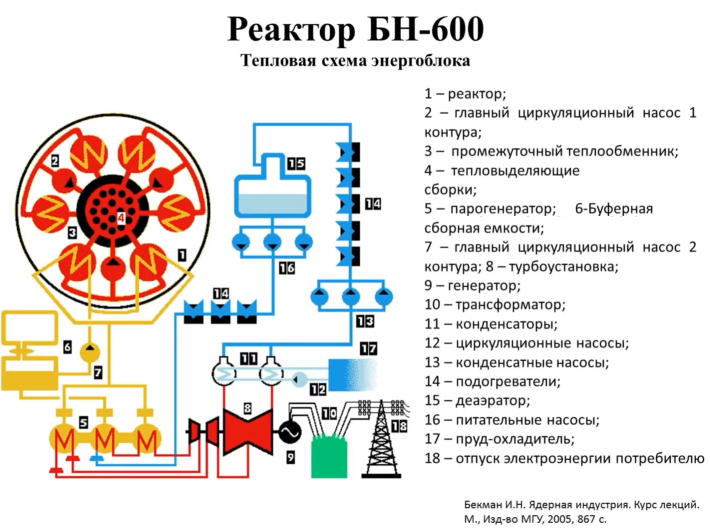
\includegraphics[width=1\linewidth]{pics/bn}
	\caption{Схема энергоблока реактора на быстрых нейтронах}
	\label{fig:bn}
\end{figure}

Высокая химическая активность натрия порождает ряд специфических проблем. Изучение возможных последствий подобных аварий, их моделирование, а также запуск всевозможных расчетов являются важным направлением анализа безопасности установок с натриевым теплоносителем. С этой целью была разработана программа моделирования, визуализации результатов расчетов и настройки компонентов гидродинамики многокомпонентной смеси blleak16d.

Вычислительные программы, используемые для моделирования сложных физических процессов, в том числе и blleak16d, имеют большое количество различных конфигурационных и выходных файлов, которые в свою очередь содержат значительное количество разнообразной информации. 

Каждый файл конфигурации имеет сложную структуру. Один файл может содержать ссылки на несколько других и так далее. В свою очередь, в файлах содержится много однотипной и повторяющейся информации. Это значительно усложняет процесс анализа данных, если проводить его вручную.
Для облегчения анализа данных, имеет смысл провести визуализацию, которая позволит наглядно увидеть переломные моменты моделирования, т.е. моменты, в которых произошла моделируемая авария. 

Для визуализации, требуется сначала выбрать определенные параметры и переменные для вывода. Сделать это вручную, опять же, было бы очень проблематично из-за сложной иерархии файлов и большого объёма данных. Целью данной научно-исследовательской работы как раз выступает создания приложения с графическим интерфейсом, которое бы облегчило процесс подготовки к визуализации. А в последующем, могло бы и проводить саму визуализацию расчетных данных. 



\subsection{Структура конфигурационных и выходных вычислительных файлов}

Перед тем, как приступить к написанию пользовательского приложение, надо проанализировать структуру файлов, с которыми будет работать это приложение. 

В качестве основных файлов, который задают параметры контура, можно выделить:
\begin{itemize}
\item mainconf.txt – этот файл содержит в себе базовые параметры для всей системы и названия основных конфигурационных файлов, в которые входят файлы с параметрами узлов, каналов и временного сценария;
\item bounds.txt – этот файл включает в себя информацию о количестве узлов и список всех узлов системы со ссылкой на конфигурационный файл для каждого узла;
\item timescen.txt – этот файл хранит данные временного сценария процесса моделирования;
\item chanprof.txt – этот файл содержит в себе информацию о каналах, их количестве и геометрии каждого канала, а также хранит ссылки на файлы конфигурации каналов.
\end{itemize}

Все файлы представляют собой сложную структуру, т.к. помимо описания общей информации они содержат названия других файлов, содержимое которых, в свою очередь, является также немаловажным.

Основная информация, используемая для анализа, хранится в файлах с описанием узлов, каналов, геометрии и т.д. Все данные в этих файлах хранятся в виде таблиц с заданной структурой. Каждый такой файл представляет собой массивную таблицу данных без названия полей и четкой границы столбцов. 

Кроме конфигурационных файлов, в ходе работы вычислительной программы появляются выходные расчётные файлы. Основным их содержимым являются численные данные, записанные по столбцам, которые представляют собой основную расчётную информацию и результаты снятия показаний в контуре во время протекания реакции. Сложность анализа таких данных заключается в том, что столбцы файла не имеют названий, а разделителем данных по столбца является символ пробела. Учитывая, что один такой файл имеет очень большой объём информации, выбор данных пользователем напрямую является нерезультативным и отнимает много времени. 


Чтобы более наглядно представить структуру конфигурационных и выходных вычислительных файлов, можно посмотреть на рисунок~\ref{fig:scheme}, на которой представлена иерархия этих файлов. 

\begin{figure}[H]
	\centering
	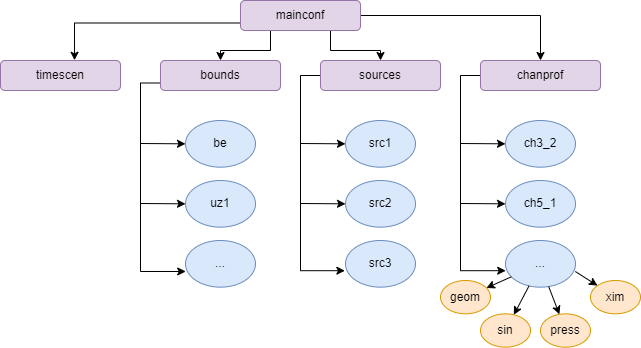
\includegraphics[width=1\linewidth]{pics/scheme}
	\caption{Иерархическая структура файлов}
	\label{fig:scheme}
\end{figure}

По вышеперечисленным причинам, необходимо разработать приложение, которое сможет считывать и обрабатывать файлы такого рода и предоставлять информацию в удобном для пользователя формате, для того, чтобы потом легко выбрать нужные параметры для визуализации. 


